\documentclass[12pt]{article}
% Packages
\usepackage[utf8]{inputenc}
\usepackage{hyperref}
\usepackage[T1]{fontenc}
\usepackage{csvsimple}
\usepackage{verbatim}
\usepackage{graphicx}
\usepackage[section]{placeins}
\graphicspath{ {/home/Users/Theo/dev/porjetMemoire/LateX/} }
% Settings and data
\hypersetup{
    colorlinks=true,
    linkcolor=blue,
    filecolor=magenta,      
    urlcolor=cyan,
    pdftitle={Overleaf Example},
    pdfpagemode=FullScreen,
    }



\title{\vspace{-3cm}{Rapport sur les travaux de mon mémoire}}
\author{Theophile Miailhe}
\date{1/04/22}

\begin{document}
\maketitle

\section{Le travail accompli :}
\paragraph*{}
Grâce à la disponibilité en format CSV de la base de données des morts en opération extérieure, je n'ai pas eu besoin de faire un scrapping du site du SHD. J'ai téléchargé les données directement de ce lien: \url{https://www.memoiredeshommes.sga.defense.gouv.fr/fr/arkotheque/navigation_facette/index.php?f=opendata}. J'ai procédé à un traitement de la  base « Militaires décédés sur les théâtres d'opérations extérieurs (1905-1962) » avec la librairie \textbf{Pandas} de \textbf{Python}. La base comportait 20.059 entrées qui correspondaient chacune à un militaire mort.  
\begin{figure}[h]
    \centering
    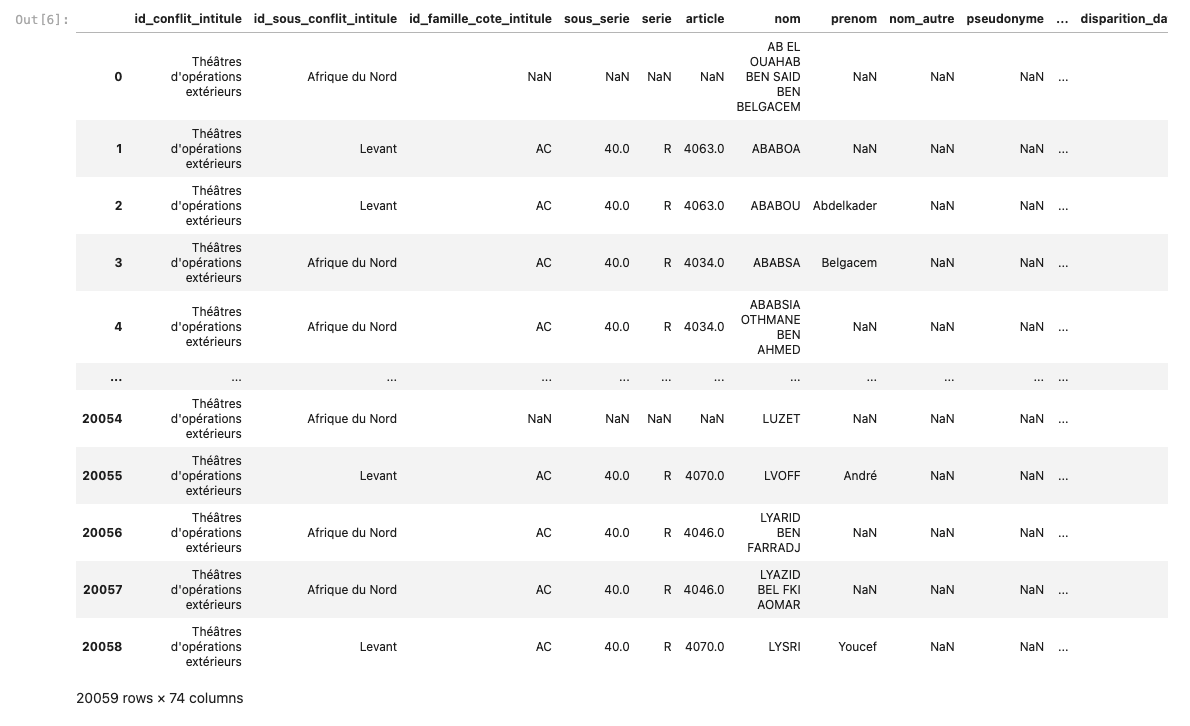
\includegraphics[scale=0.27]{dbpic.png}
    \caption{Base de données originelle}
    \label{fig:Base d'origine}
\end{figure}
\paragraph*{}
Ensuite j'ai filtré la base par année et par lieu de décès. La période qui m'intéresse est de janvier 1925 à décembre 1926 où la majorité des combats ont eu lieu. Dans la base, il y a une colonne pour le pays de décès et là j'ai filtré pour le Maroc. Le script que j'ai utilisé pour filtrer la base se trouve sur la \textbf{branch v.02} de mon projet sur \href{https://github.com/the0phil3/projetMemoire/tree/v.02}{Github}. Ce travail m'a permis de créer une base de données personnelle des sujets qui m'intéressent :
\begin{figure}[h]
    \centering
    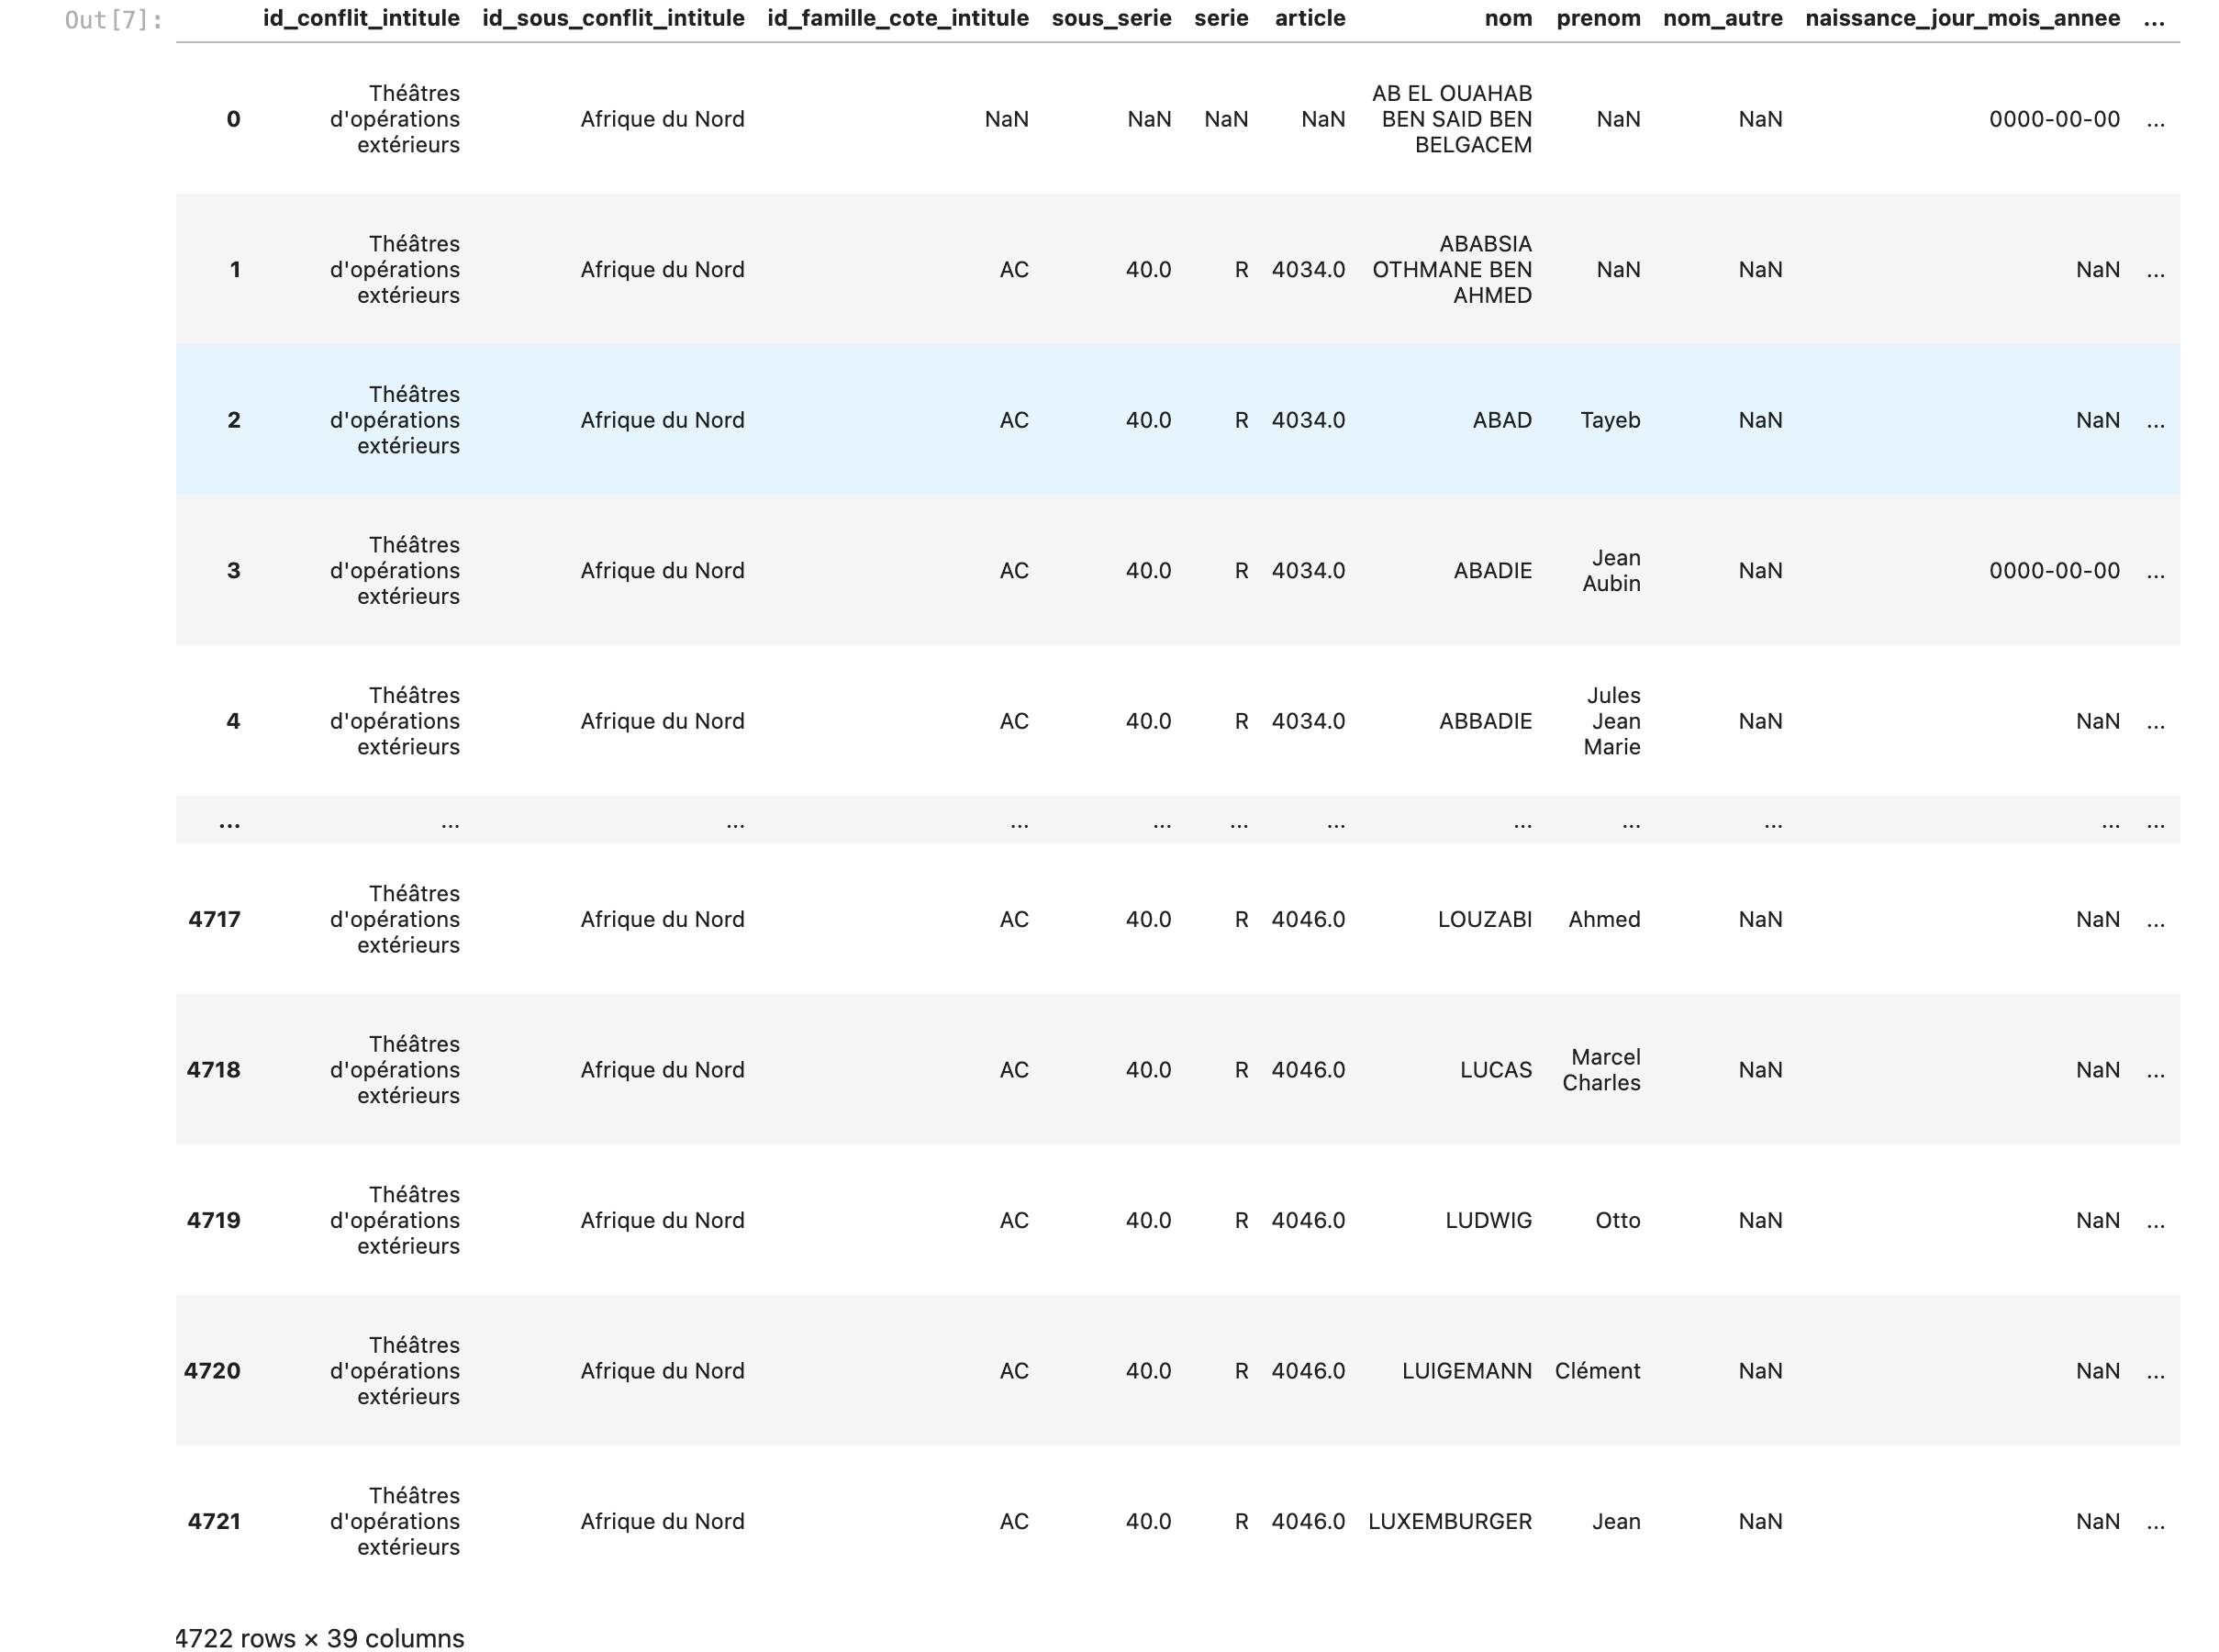
\includegraphics[scale=0.27]{mortsduRif.png}
    \caption{Base de données finale}
    \label{fig:Base finale}
\end{figure} 
\paragraph*{}
Avec cette base constituée, j'ai commencé les premières manipulation des caractéristiques des soldats telles que leur régiment ou leur lieu de décès. Mon but était de faire une pré-analyse avant de commencer à traiter les soldats par nom et faire l'OCR des fiches matricules. Le script que j'ai utilisé pour faire mes premières figures se trouve la \textbf{branch v.03} de mon projet sur \href{https://github.com/the0phil3/projetMemoire/tree/v.03}{Github}. J'ai chercher les 20 régiments avec le plus de pertes et les 20 lieux avec le plus de morts dans ma base :
\begin{figure}[!ht]
	\centering
    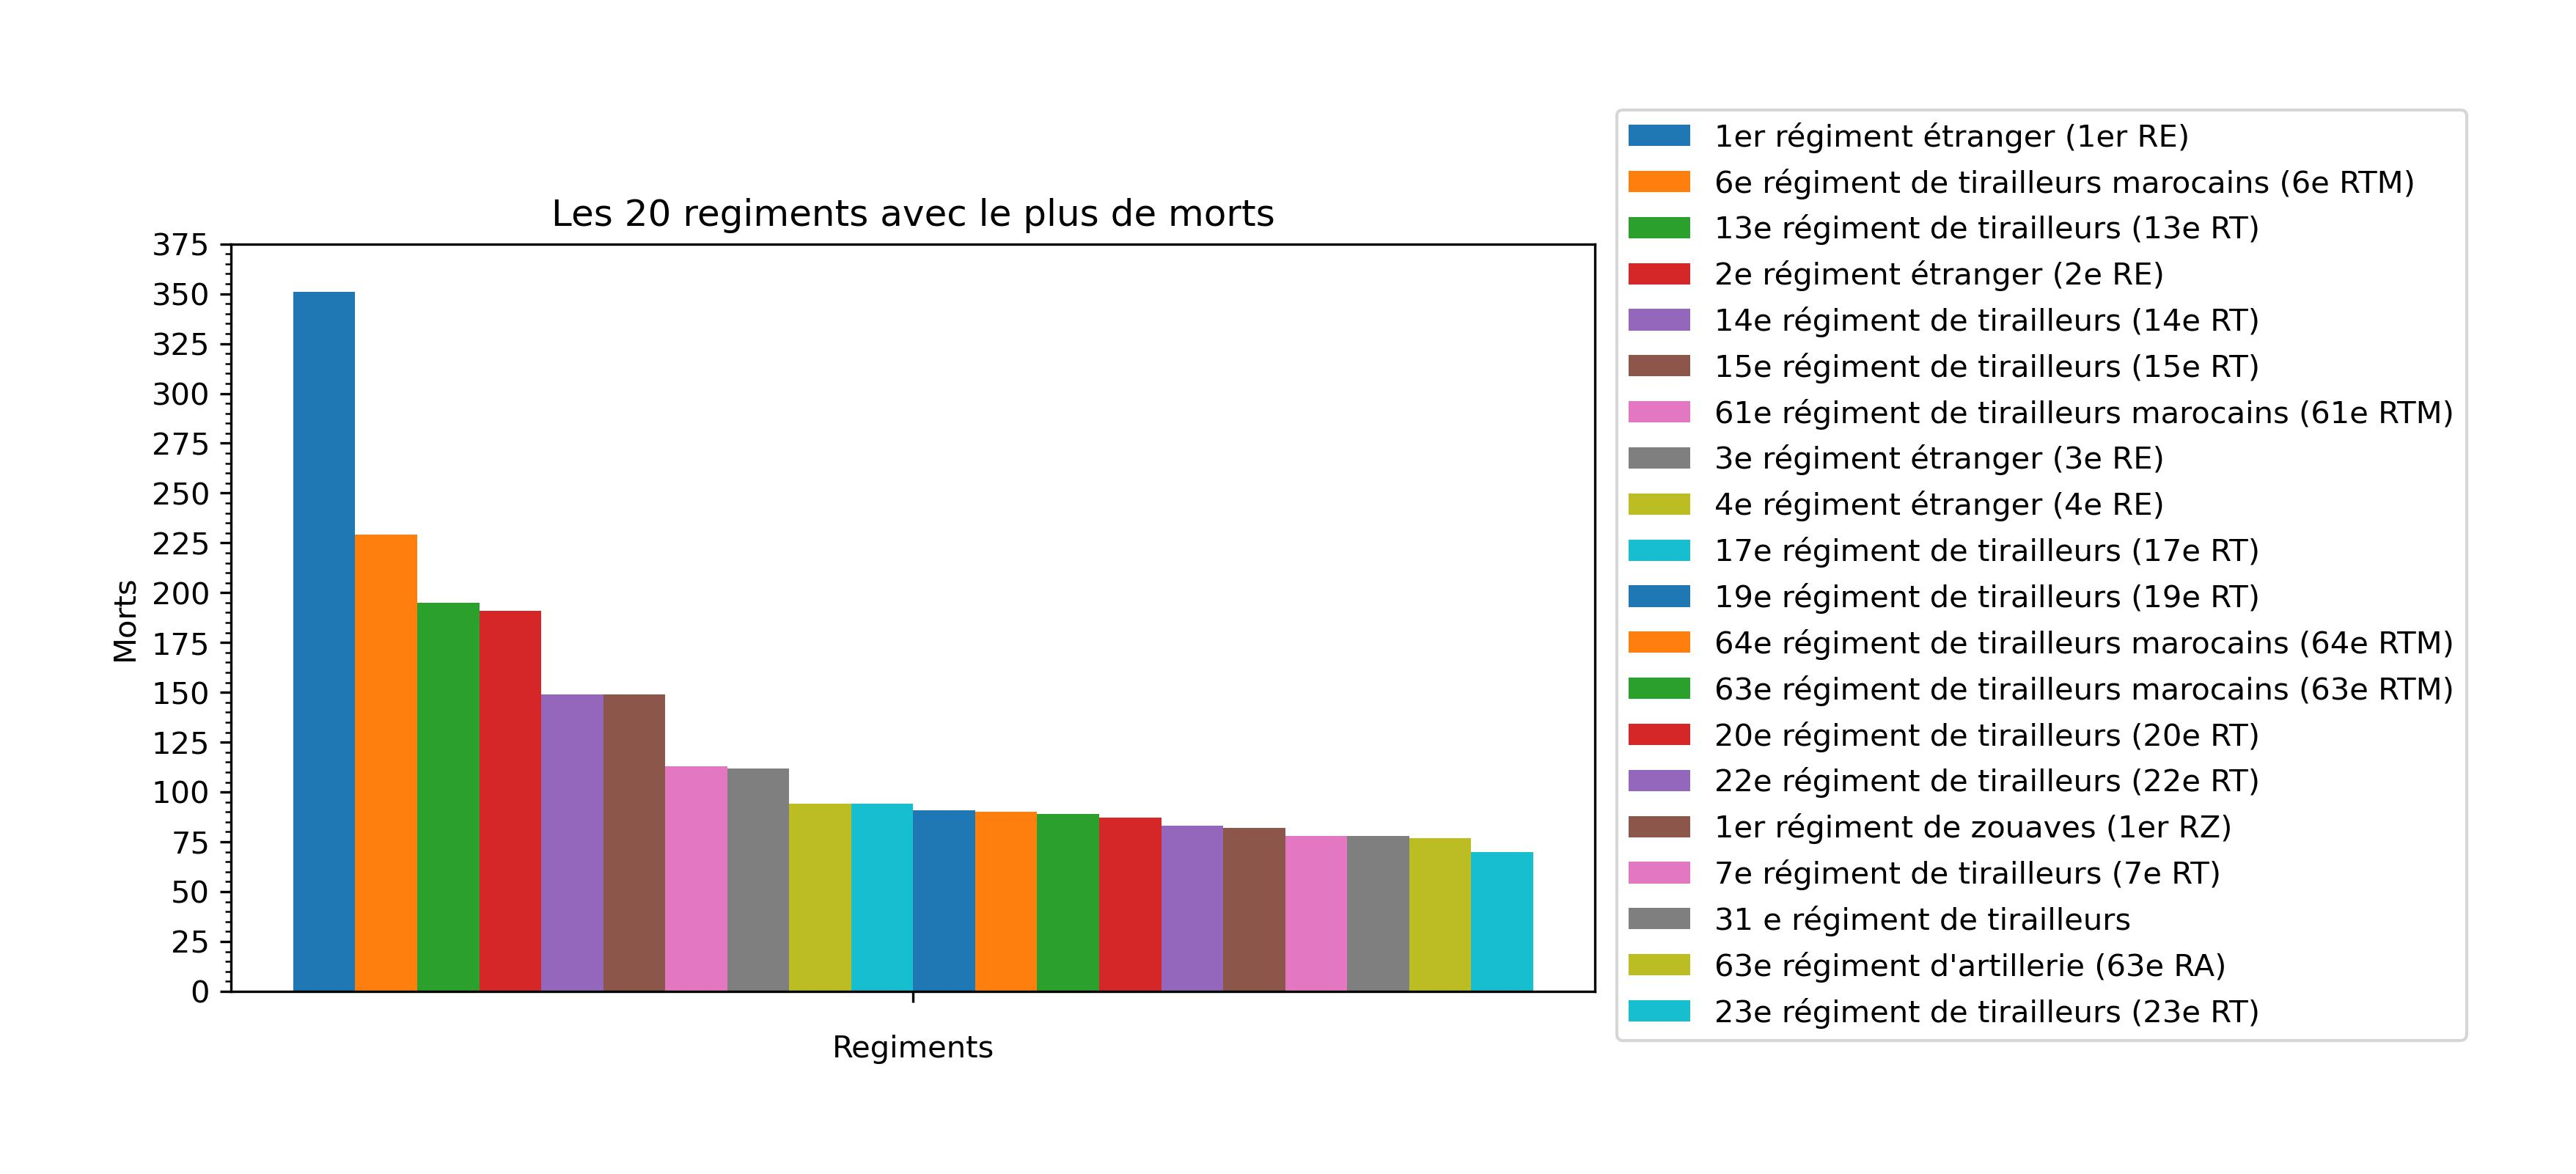
\includegraphics[scale=0.6]{20regiments.jpg}
    \caption{Les 20 premiers régiments avec le plus de morts}
    \label{fig:20regiments}
\end{figure}  
\begin{figure}[!hb]
	\centering
    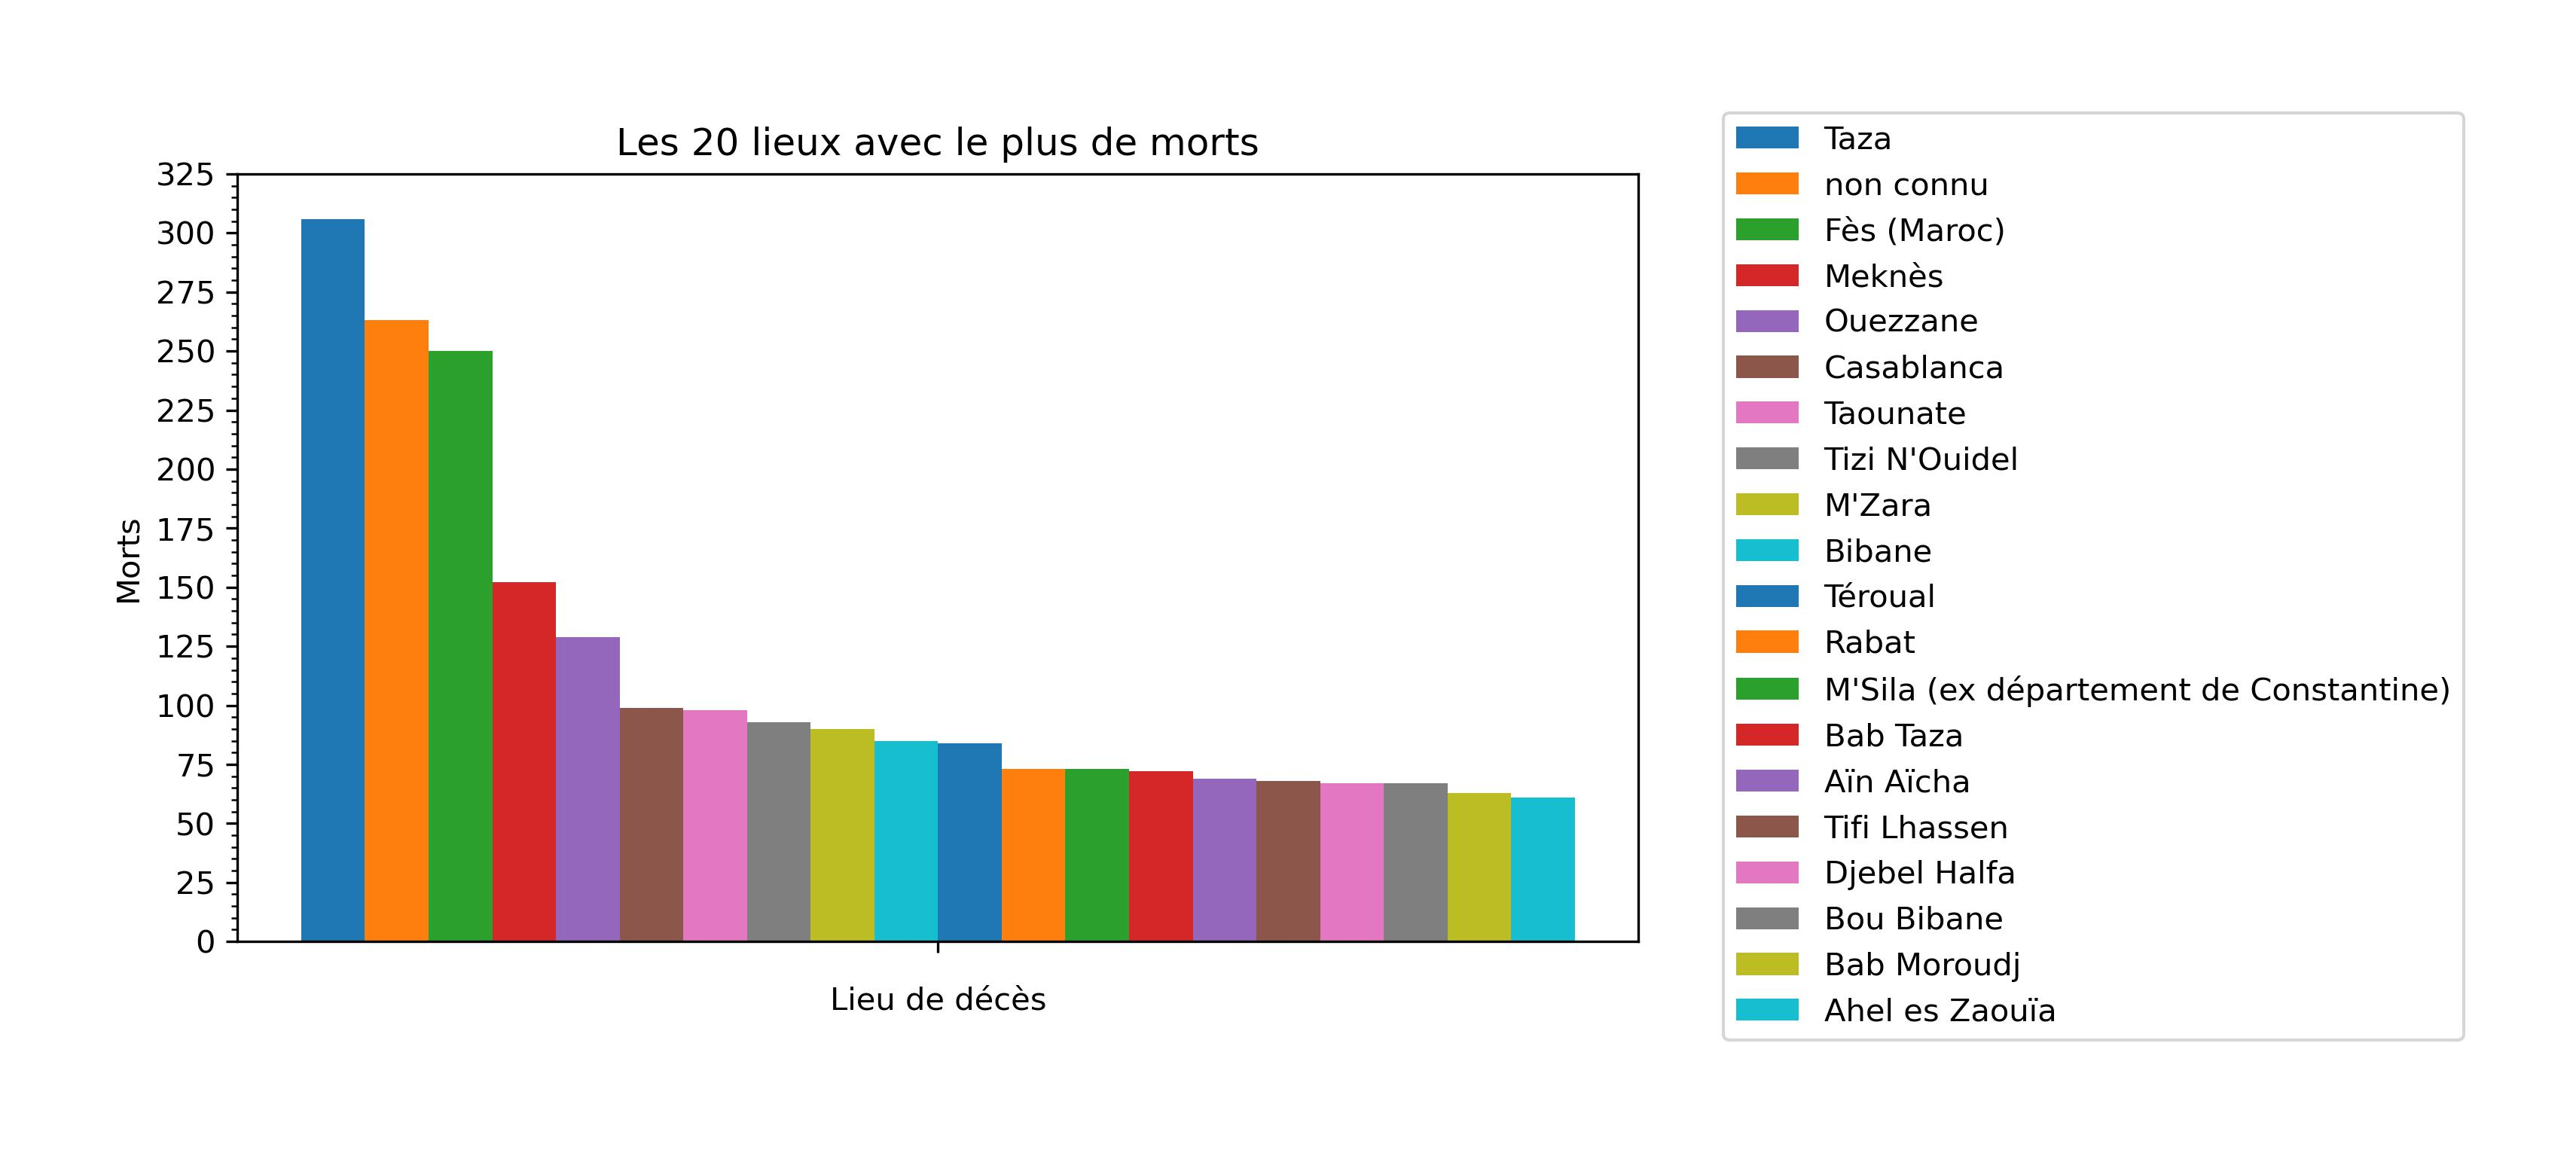
\includegraphics[scale=0.6]{20places.jpg}
    \caption{Les 20 premiers lieux avec le plus de morts}
    \label{fig:20places}
\end{figure}  

\section{Les problèmes :}
\paragraph*{}
Le premier problème qui m'a interpellé est la vérification de mes données avec celles Max Schiavon dans son ouvrage \emph{La guerre du Rif}. Je partage ici un scan de l'ouvrage de Schiavon qui décrit les pertes de l'armée avant l'offensif rifaine de 1925.\cite{Schiavon}
\begin{figure}[!htb]
	\centering
    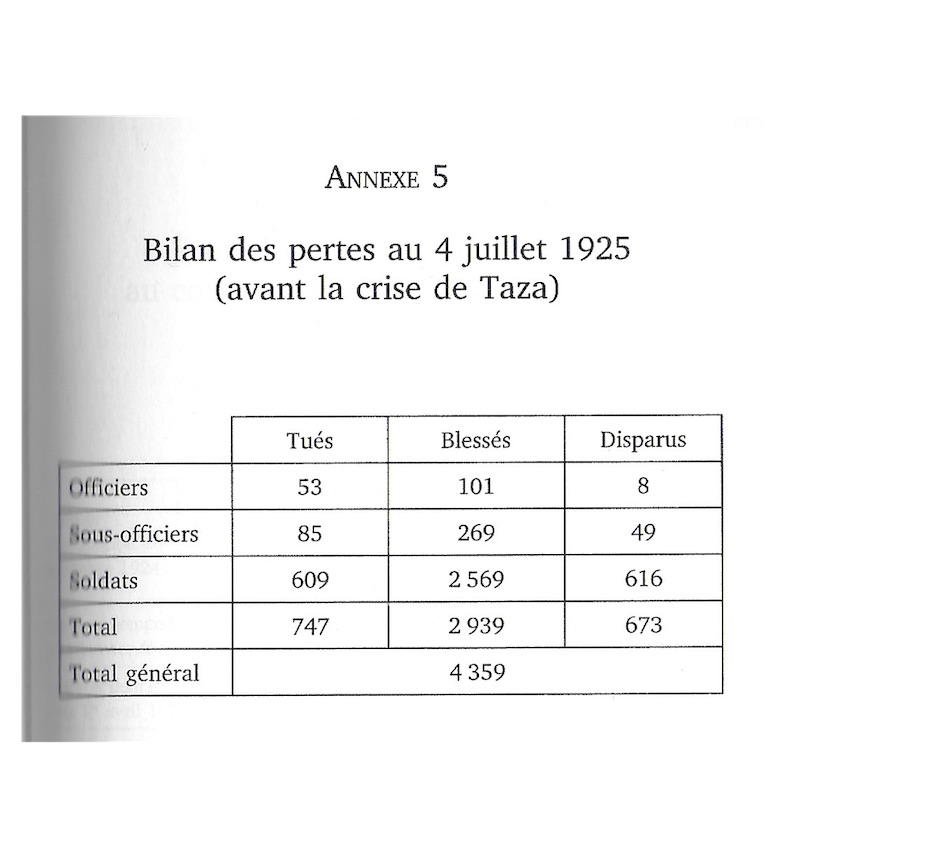
\includegraphics[scale=0.4]{schiavon.jpeg}
    \caption{Bilan de pertes 1925}
    \label{fig:schiavonscan}
\end{figure}  Dans le support de son ouvrage, il inclut beaucoup de données quantitatives sur la guerre mais pas le bilan des pertes totales. Donc il faudrait que j'essaie de trouver dans quel référence au SHD il a trouvé ces chiffres.   

\paragraph*{}
Je me suis aussi rendu compte en créant mes premières figures que la base de données était pas forcement très propre. J'ai trouvé déjà un cas d'un double de la même personne et dans la Figure 4 vous pouvez voir qu'il y a « M'Sila » qui est en Algérie et pas au Maroc. Il faudrait que je trouve un moyen de filtrer les doubles et procéder à une vérification des noms de lieu. 
 
\section{Le travail à faire :}
\paragraph*{}
Maintenant que j'ai ma base constituée, il faut: \begin{enumerate}
\item La nettoyer
\item Contacter le SHD pour vérifier l'origine des données chiffrés 
\item Trouver une méthode pour diviser les soldats par origines 
\item Constituer mon échantillon des fiches matricules numérisées
\item Commencer l'OCR des fiches matricules et vérifier sa faisabilité
\end{enumerate}


\listoffigures

\begin{thebibliography}{1}
\bibitem{Schiavon}
Max Schiavon, (1986) \emph{La guerre du Rif - Un conflit colonial oublié (1925-1926)}, Éditions Pierre de Taillac, 2016, 352 pages.
\end{thebibliography}


\end{document}